\documentclass[10pt]{article}
\usepackage[preprint]{tmlr}
\usepackage{graphicx}
\usepackage{booktabs}
\usepackage{amsmath,amssymb}
\usepackage{hyperref}
\usepackage{url}
\usepackage{bm}

\title{SpectraLoRA: Post-Training Compact Molecular Foundation Models for  Surrogate Raman Prediction and Post-Hoc Spectral Alignment via Structural Prompting and Derivative-Free Optimization}

\author{\name Rahul Khorana \email rahul.khorana@arcadiascience.com \\
\addr Arcadia Science}

\def\month{03}
\def\year{2026}
\def\openreview{\url{https://openreview.net/forum?id=XXXX}}

\begin{document}

\maketitle

\begin{abstract}
Raman spectroscopy has become increasingly prevalent as a tool for scientists to interrogate molecules. However, the cost and time required to determine spectra for millions of compounds when screening for drug-like candidates is prohibitive. Moreover, approximations such as DFT-based vibrational analysis suffer from computational efficiency and scaling issues dependent on the chosen exchange-correlation functional. Simultaneously, machine learning methods have become increasingly reliable as data has become more readily available. In this manuscript, we present a scalable, robust, domain-adaptive pipeline for post-training chemical foundation models that can perform approximate vibrational analysis. We curate a large dataset of approximately 22 million molecules, along with their molecular geometries, quantum-mechanical properties, and DFT-simulated Raman spectra. We develop a scalable distributed system for training foundation models on this dataset. We design a parameter-efficient foundation model for peptides and small molecules that can predict Hessians, vibrational frequencies, and approximate Raman spectra from 3D atomic coordinates. We provide a fine-tuning and ``alignment'' strategy leveraging $\mathrm{SO}(3)$-Equivariant Graph LoRA, and Derivative-Free Optimization to adapt the model to downstream Raman prediction tasks. We evaluate the model on an entirely out-of-distribution benchmark consisting of larger peptides with DFT-simulated spectra and a separate set of experimentally measured spectra. We demonstrate our model performs, in a zero-shot setting on an out-of-distribution dataset, comparably to a state-of-the-art model evaluated entirely on in-distribution molecules. The entire framework lays the foundation for a kind of ``Sim-to-Real'' transfer, in which one starts with a frozen model trained on simulated data and adapts it to make high-fidelity predictions on real-world experimental data, even when the target domain is structurally and chemically distinct from the training domain.
We report a model capable of recovering $67.2\%$ of DFT-simulated modes in the fingerprint region within $\pm 10$~cm$^{-1}$ with a median positional error of $3.56$~cm$^{-1}$. The primary limitation remains intensity prediction (${\sim}7\times$ error), which we partially overcome via post-hoc spectral alignment using NES, pushing fingerprint F1@15 from 0.426 to 0.532 and peak recall to 0.703, thereby exceeding the in-distribution recall of Mol2Raman (0.634) on a harder out-of-distribution benchmark.
\end{abstract}

%% ====================================================================
\section{Introduction \& Background}
\label{sec:introduction}
%% ====================================================================

\paragraph{Raman Spectroscopy} Francis Bacon, first Viscount St Alban, allegedly wrote, ``Am Anfang war das Spektrum; dann kam das Fitten.'' If not Bacon, then at least Raman spectroscopy follows a similar principle: what is hidden in matter is brought into evidence by light, though not without obscurity. Stated more accurately, Raman Spectroscopy is a non-destructive technique that provides a unique chemical fingerprint based only on the interaction of light with a sample \citep{avasthi2024raman, braverman2025diy}. Raman Spectroscopy is increasingly used in Biology due to its Label-free nature \citep{han2012label}. It can reveal molecular composition, structure, and environmental information \citep{braverman2025diy}. At Arcadia Science, Raman Spectroscopy is used for inferring complex phylogenetic relationships among diverse microbial taxa, biological phenotyping, and collecting spatially resolved biochemical data on yeast cells \citep{avasthi2023raman, bulow2026coherent, essock2025comparison}. Raman Spectroscopy is also widely used in materials science and pharmaceutical development \citep{gala2015principles,neuville2014advances}. In drug discovery, Raman Spectroscopy can be used for chemical identification, preformulation, solid form screening, and bioanalysis \citep{paudel2015raman}. However, experimentally determining spectra for millions of compounds when screening for drug-like candidates is expensive and time-consuming \citep{cutshaw2023emerging, sorrentino2025mol2raman}. Moreover, leveraging DFT-methods to calculate vibrational spectra can, depending on system and exchange-correlation functional, lead to high computational cost and scaling issues \citep{taherivardanjani2022benchmarking, bremond2026contemporary}.

Raman spectroscopy is then understood to be a technique used to investigate the vibrational structure of molecules. Raman Scattering, however, is a two-photon process distinct from Rayleigh Scattering \citep{herman2003raman}. Rayleigh Scattering is simply quasielastic scattering by nonpropagating density changes caused by entropy fluctuations \citep{herman2003raman}. Raman Scattering is, contrastingly, the inelastic scattering of electromagnetic radiation, which in quantized form consists of photons. Stated classically, Raman Scattering is a two photon process involving an interaction with an incident radiation that makes the molecule explore a virtual state, namely a superposition of excited states, and the emission of a photon with energy that differs from the incident one by a molecular vibrational frequency \citep{dall2022time}. In Rayleigh Scattering the scattered photon brings the molecule back to the initial state. Alternatively, theory developed by \citet{lee1979time} justified a view of the Raman process as result of the propagation of a wavepacket on the excited-state potential energy surface. Raman Intensity is then determined by the half Fourier Transform of the overlap of initial and final states \citep{lee1979time, heller1982simple}. Methods employed to simulate Raman scattering start from the Kramers, Heisenberg, and Dirac polarizability tensor and can be categorized in time-independent and time-dependent strategies \citep{kramers1925streuung,dall2022time}. However, we prefer time-dependent strategies expressed through the lucid treatment developed by \citet{dall2022time}. Summarized succintly through the framework of perturbation theory applied to the two-photon formula by \citet{dall2022time} the initial wave function and electric field induces dynamics on an excited PES expressed as
\begin{equation}
| \Psi^{(1)}(t)\rangle = i \int_{-\infty}^t dt' e^{-i\hat{H}(t-t')}\hat{\vec{\mu}} \cdot \vec{\epsilon}_{I}(t') e^{-iE_0t'}| \Psi_0(-\infty)\rangle 
\end{equation}
in atomic units. Here, $\Psi_0(-\infty)\rangle$ is the unpeturbed wave function with energy $E_0$, $\hat{\vec{\mu}}$ the transition dipole moment operator, and $\vec{\epsilon_{I}}(t')$ the incident electric field. $\hat{H}$ is the sum of the nuclear and electronic Hamiltonians in the Born-Oppenheimer approximation. \citet{dall2022time} account for spontaneous emission from the vritual state by introducing a classical field $\vec{\epsilon}_S$ at monochromatic frequency $\omega_S$ wherein at the second order we get 
\begin{equation}
| \Psi^{(2)}(t, \omega_S)\rangle = \frac{i}{2} \int_{-\infty}^t dt' e^{-i\hat{H}(t-t')}\hat{\vec{\mu}} \cdot \vec{\epsilon}_S e^{i\omega_S t'}| \Psi^{(1)}(t')\rangle
\end{equation}
Then writing the wave function as a linear combination of vibronic eigenstates $|J\rangle$ and making some substitutions,we can determine the time-dependent coefficients of the state $N$ as
\begin{equation}
\langle N | \Psi^{(2)}(t, \omega_S)\rangle = \frac{i}{2} \int_{-\infty}^t dt' \langle N | e^{-i\hat{H}(t-t')} \hat{\vec{\mu}} \cdot \vec{\epsilon}_S e^{i\omega_S t'}| \Psi^{(1)}(t')\rangle
\end{equation}
The second order wave function coefficients of a state $N$ at the limit $t \to \infty$ is exactly the Inverse Fourier Transform with respect to the scattered frequency of the first order coefficients, that is directly related to the Raman scattering intensity \citep{dall2022time}.

\paragraph{DFT \& Limitations} The most widely used and practical implementation of Density Functional Theory (DFT) is Kohn-Sham Density Functional Theory (KS-DFT). KS-DFT is a computational framework for modeling electronic structure. The initial assumption when working with DFT is based on either the atomic orbitals or plane-wave basis sets \citep{epifanovsky2021software, frisch2016gaussian}.

\citet{hohenberg1964inhomogeneous} in their namesake theorem showed that if $N$ interacting electrons move in an external potential $V_{\text{ext}}(r)$ the ground state electron density $n_0(r)$ minimizes the functional
\begin{equation}
    E[n] = F[n] + \int n(r) V_{\text{ext}}(r)  dr
\end{equation}
where $F$ is a universal functional of $n$ and $E_0$ the exact ground-state electronic energy \citep{kent1999techniques}.

\citet{kohn1965self} derived a coupled set of differential equations enabling the ground state density $n_0({r})$ to be found. $F[n(r)]$ was separated so that $E$ becomes
\begin{equation}
E[n] = T_s[n] + \frac{1}{2} \int \int \frac{n(r) n(r')}{|r-r'|} dr dr' + E_{\text{XC}}[n(r)] + \int n(r) V_{\text{ext}}(r) dr
\end{equation}
where $T_s[n]$ is the kinetic energy of a non-interacting electron gas with density $n({r})$ \citep{kent1999techniques,kohn1999nobel}. Simply stated
\begin{equation}
T_s[n(r)] = -\frac{1}{2}\sum_{i=1}^N \int \psi_i^{\ast}(r) \nabla^2 \psi_i(r) dr
\end{equation}.
Inducing a normalization constraint on the electron density $\int n(r) dr = N$ we see $\frac{\delta E[n(r)]}{\delta n(r)} = \mu$. Thusly, re-writing in terms of the effective potential
\begin{equation}
\begin{aligned}
\frac{\delta T_s[n(r)]}{\delta n(r)} + V_{\text{eff}}(r) &= \mu \\
\text{such that} \qquad
V_{\text{eff}}(r) &= V_{\text{ext}}(r)
+ \int \frac{n(r')}{|r - r'|}\,dr'
+ V_{\text{XC}}(r)
\end{aligned}
\end{equation}
To find the ground state energy, $E_{0}$, and the ground state density, $n_0$, the one electron Schrödinger equation
\begin{equation}
\left( -\frac{1}{2} \nabla^2_i + V_{\text{eff}}(r) - \epsilon_i \right)\psi_i(r) = 0
\end{equation}
which should be solved self-consistently with 
\begin{equation}
n(r) = \sum_{i=1}^{N} |\psi_i(r)|^2
\end{equation}
as intended. The theorem of Hohenberg and Kohn is the typical justification for DFT \citep{penz2023structure}. As we are aware, in essence, the theorem states that the one-body particle density uniquely, up to additive constant, determines the scalar potential of a nonrelativistic many-electron system in its ground state \citep{penz2023structure,hohenberg1964inhomogeneous,kohn1999nobel}. However, the work of Lieb raised questions regarding the differentiability of the involved functionals that map densities to energies \citep{lieb2013current,lammert2007differentiability,penz2023structure}. \citet{lammert2007differentiability} demonstrated that the key functional of DFT is indeed nondifferentiable. Moreover, it was determined that it is not always the case that electron densities of real physical systems are always noninteracting $v$-representable \citep{trushin2024violations}. The Kohn-Sham approach fundamentally relies on the assumption that the density is simultaneously interacting and non-interacting $v$-representable \citep{sutter2024solution}. Additionally, popular approximations like LDA or GGA are inadequate to predict the band
gap of solids, or the correct dissociation of heteroatomic molecules \citep{Perfetto_2012}. The conceptual advance to addresss these issues was ensemble-DFT \citep{gould2026ensemblization}. The discontinuity in $\frac{\partial E}{\partial N}$ is usually the difference between the ionization energy and the electron affinity \citep{Perfetto_2012}. Within the KS formalism the relationship between KS energy levels and many-electron energies is not straightforward \citep{kraisler2021kohn}. While, for the exact KS potential the highest occupied (ho), the KS energy level $\varepsilon^{(\text{ho})}$ equals minus the IP, the fundamental gap does not simply equal the KS gap, instead they differ which is termed derivative discontinuity \citep{kraisler2021kohn}. While the HK setting is tied to ground state densities and potential uniqueness under nondegeneracy assumptions, Lieb's formulation cleverly places the theory in a Banach-space setting and identifies the exact density functional as the convex dual of the ground-state energy viewed as a functional of the external potential \citep{sheng2026exactdensityfunctionaltheoryparallel,lieb2013current}. Simply put, let $H[v]$ be the standard non-relativistic electronic Hamiltonian, define $T = -\frac{1}{2} \sum_{i=1}^N \Delta_i$, $W = \sum_{1 \leq i < j \leq N} \frac{1}{|r_i - r_j|}$, and $V[v] = \sum_{i=1}^{N} v(r_i)$. Then as shown by Lieb, the exact interacting universal functional is defined by
\begin{equation}
F[\rho] = \inf_{\Gamma \mapsto \rho} \text{Tr}\left( \Gamma(T + W) \right)
\end{equation}
where $\Gamma$ ranges over positive trace-class operators with $\text{Tr}(\Gamma) = 1$ \citep{sheng2026exactdensityfunctionaltheoryparallel}. Alternatively, one may be more familiar with the Levy-Lieb functional as presented:
\begin{equation}
\begin{split}
F_{\text{LL}}[\rho]
= \inf_{\substack{
    \Psi \in \wedge_{i=1}^{N} L^{2}(\mathbb{R}^{d} \times \mathbb{Z}_q, \mathbb{C}) \\
    \|\Psi\|_{L^2}=1,\ \rho_\Psi = \rho
}}
\left\{
    \frac{1}{2} \sum_{j=1}^N
    \int_{(\mathbb{R}^d \times \mathbb{Z}_q)^{N}}
    |\nabla_j \Psi(X)|^2 \, dX
\right.\\
\left.
    + \sum_{1 \leq j < k \leq N}
    \int_{(\mathbb{R}^d \times \mathbb{Z}_q)^{N}}
    |\Psi(X)|^2 \omega(r_j-r_k)\, dX
\right\}
\end{split}
\end{equation}
\citep{mietzsch2020validity, levy1979universal, lieb2013current}.

\paragraph{Chemical Foundation Models}
\citet{foundationmodels} describe foundation models as  models trained on broad data, generally using self-supervision,that can be adapted to a wide range of downstream tasks. Typically one imagines foundation models to contain billions of parameters and leverage MoE, FlashAttention mechnaisms, and some flavor of RLHF/DPO/GRPO see \citet{deepseekai2024deepseekv2strongeconomicalefficient} for one such example.
In chemistry however, the notion of a foundation model is inherently different. For one, molecules are not best represented by tokens \citep{guo2023graphbasedmolecularrepresentationlearning, khorana2024polyatomiccomplexestopologicallyinformedlearning, Krenn_2020, langer2022representations}. Geometric constraints are more appropriate when working with molecules \citep{NEQUIP, fu2023learning, musaelian2023learning, batatia2022mace,ALLEGRO-FM}. The most important, in our opinion, chemical foundation models are the MACE-MP/MACE-OFF series, GRACE-2L series, NequIP derivatives such as NequIP-OAM-L, PET, and Allegro-FM \citep{MACE-MP, GRACE-2L, NEQUIP,ALLEGRO-FM, PET}. 

\paragraph{MACE-MP} MACE-MP is a foundation model for atomistic materials chemistry \citep{MACE-MP}. MACE-MP is built off of the MACE architecture which is an equivariant graph based model \citep{batatia2022mace}. MACE-MPA-0 has 9.06M parameters.

\paragraph{GRACE-2L} GRACE is a foundational machine learning interatomic potential leveraging Graph Atomic Cluster Expansion \citep{GRACE-2L}. GRACE-2L-OAM-L, the largest variant at this time, has approximately 26.4M parameters. GRACE-2L-OAM has 12.6M parameters, and GRACE-1L-OAM has 3.45M parameters.

\paragraph{NEQUIP-OAM} Neural Equivariant Interatomic Potentials, are a class of graph neural network (GNN) models used for atomistic simulations in materials science and chemistry \citep{NEQUIP}. NequIP is the backbone model for a few later foundation models such as NequIP-OAM (9.6M parameters), NequIP-OAM-XL (32.1M parameters), ReaxNet, and Nequix (700K parameters) \citep{gao2025foundation,koker2025training}.

\paragraph{ALLEGRO-FM} ALLEGRO-FM is a large-scale equivariant graph-based foundation model for exascale molecular dynamics \citep{ALLEGRO-FM}. The largest variant, Allegro-FM512, has 2.6M parameters. The smaller variants, Allegro-FM256 and Allegro-FM64, have 690k and 44k parameters respectively.

\paragraph{PET} One of the most recent developments in this space has been the UPET/PET family of models, which are designed to be universal atomistic models. PET-OAM-XL has 700M parameters, PET-MAD has 2.8M parameters \citep{PET}.

Traditionally chemical foundation models are graph based, equivariant networks trained on large datasets and are, relatively speaking, parameter efficient, and orders of magnitude smaller than recent LLMs. Many use some flavor of LoRA see for instance \citet{PET}. More recently, the rather famous Head-Gordon Lab at Berkeley, within the last several weeks, laid out more specific criteria for what constitutes a successful MLIP or chemical foundation model \citep{yuan2026foundation}. They state, ``A successful MLIP Foundation Model for atomistic simulation should perform well on a diverse range of tasks after finetuning and post-training, spanning different levels of theory, different types of systems, static and dynamic quantities, and a range of properties beyond just energies and forces'' \citep{yuan2026foundation}. We will evaluate our model using only some of these metrics and establish a slightly different yardstick.


\paragraph{Pre-Training, Post-Training \& SFT} 
The Post-Training literature is rather vast. We will briefly cover a few of the most popular paradigms and techniques. \citet{grattafiori2024llama} when training the LLaMA3 models outline a well-adopted strategy when post-training. Usually, foundation model development consists of two stages: pre-training in which the model is exposed to a massive corpus on a simpler objective such as next-word prediction, and in the second stage, the model is tuned to follow instructions and align with human preferences \citep{grattafiori2024llama}.
\begin{itemize}
    \item \textbf{Pre-training} In NLP, pre-training involves converting a large, multilingual text corpus into discrete tokens and performing next-token prediction. Historically, this has been done via being provided an unsupervised corpus $\mathcal{U} := \{u_1, \ldots, u_k\}$ wherein we use standard the standard language modeling objective to maximize $\sum_i \log(P(u_i ~|~ u_{i-k}, \ldots, u_{i-1}, \theta))$ \citep{radford2018improving}. In more modern settings, the standard pre-training stage is followed by a continued pre-training stage that increases the supported context window \citep{grattafiori2024llama}. Additionally, strategies such as Position Interpolation (PI) extend the context window sizes of RoPE-based pretrained LLMs such as LLaMA \citep{chen2023extending}.
    \item \textbf{Post-training} Usually, pre-trained language models have a rich understanding of language, but do not follow instructions or behave optimally. Hence, models are aligned with humna feedback over the course of many rounds. This is achieved via Supervised Fine-Tuning (SFT) on instruction tuning data and Direct Preference Optimization (DPO) \citep{grattafiori2024llama, rafailov2023direct}. During Post-training sometimes tool-usage is introduced. Usually, one defines a reward model and language model. 
    After, one begins by training a reward model on top of the pre-trained checkpoint using some kind of preference data \citep{grattafiori2024llama}. Then, one finetunes pre-trained checkpoints with SFT \citep{grattafiori2024llama}. Finally, one can align checkpoints further with DPO \citep{grattafiori2024llama}. After training the reward model one can perform rejection sampling and even curate synthetic data with which finetuning can be performed. This is the strategy behind LLama3 \citep{grattafiori2024llama}.
\end{itemize}
Both Pre-training, Post-training, and varying approaches are covered in more depth with greater lucidity in \citet{Guo_2025}. However, more interesting research is present.
\paragraph{On SFT \& a Hypothesis} In ``LIMA: Less Is More for Alignment,'' \citet{zhou2023lima} demonstrate that almost all knowledge in large
language models is learned during pretraining, and only limited instruction tuning data is necessary to teach models to produce high quality output. Additonally, \citet{wei2022finetuned} demonstrates that instruction tuning, namely finetuning language models on a collection of datasets described via instructions, substantially improves zero-shot performance on unseen tasks. \textit{Taken together, we hypothesize that for Chemical Foundation Models (1) only a medium amount of experimental data is needed to align DFT-derived predictions of Raman spectra (2) well-annotated experimental data on less complex molecules will likely lead to reasonable in zero-shot performance even in more complex chemical domains e.g. materials or proteins provided pre-training data contains sufficiently complex DFT data}. This is, however, unproven conjecture at the moment.

\paragraph{On Alignment} The foundational pipeline for alignment was established by \citet{ouyang2022training}. Usually we:
\begin{itemize}
    \item[(1)] SFT: Collect demonstration data, let a labeler demonstrate ideal behavior, and use this data to fine-tune a language model with supervised learning. 
    \item[(2)] RM Training: We sample several model outputs and rank them from best to worst. This data is used to train our Reward model.
    \item[(3)] RL via PPO: We optimize a policy against this reward model via sampling a prompt, allowing the policy to produce output, scoring it, and updating the policy with PPO.
\end{itemize}
The more modern standard for alignment is DPO as developed by \citet{rafailov2023direct}. In DPO we:
\begin{itemize}
    \item [(1)] Sample completions $y_1, y_2 \sim \pi_{\text{ref}}(\cdot|x)$ for all prompts $x$ and label with human preferences to construct dataset $\mathcal{D} := \{(x_i, y_i, y_{\ell})^{(i)}\}_{i=1}^{N}$. 
    \item [(2)] Optimize language model $\pi_{\theta}$ to minimize $\mathcal{L}_{\text{DPO}}$ for the given $\pi_{\text{ref}}$ and $\mathcal{D}$ and desired $\beta$. (usually we initialize $\pi_{\text{ref}} = \pi^{\text{SFT}})$, if not available $\pi_{\text{ref}} := \text{argmax}_{\pi} \mathbb{E}_{(x, y_\omega) \sim \mathcal{D}}[\log(\pi(y_{\omega}|x))]$.
\end{itemize}
Our alignment paradigm, given the domain and problem setup, differs from these more standard ways of optimizing a large model to align with human preferences. Human preferences are, to a great extent, summarized by the phrase, ``Make it look like the experimental output I measured last Tuesday at noon when the ambient temperature was 22.2 celsius.''

\paragraph{Sim2Real} \citet{Sim2Real} in their monumental paper define the Sim2Real paradigm and the technique of domain randomization. 


\paragraph{Robotics \& Sim2Real} Classically Sim2Real is all about bridging the so called ``reality gap.'' \citet{Sim2Real} argue that there exists a fundamental separation from simulated robotics and experiments on hardware conducted in the real world. They go on to propose domain randomization a technique wherein a model is trained on simulated images that transfer to real images by randomizing rendering in the simulator. Their hypothesis being, that with great enough variability in the simulator comes real-world generalization, as the actual world the robot interacts with is simply another variation of the simulation \citep{Sim2Real}.

\paragraph{Science \& Sim2Real} In science, simulations are often notoriously limited. The reality gap is oftentime massive. In this regard, the question of ``How close is close enough?'' often arises. Experimentalists ask ``How much data do you need to model phenomenon X accurate to within some specified error tolerance $\varepsilon$?'' The answer inevitably being, ``Yes, more data.'' We take a more pragmatic stance when answering this question:
\begin{itemize}
    \item [(1)] Give me all the experimental data you have.
    \item [(2)]I will train a large model on the simulated data. It will be inaccurate when compared to experiment, and this is perfectly fine. {The goal here is robust zero-shot generalization within the simulation (e.g., training on small molecules or small peptides to zero-shot extrapolate to larger peptides or even proteins).}
    \item [(3)] I will fine-tune, adapt, or align the model to experimental reality with your experimental data, assuming the pre-trained model has learned enough about the underlying physics to transfer efficiently.
\end{itemize}
This somewhat relates to the $\Delta$-ML paradigm put forth by \citet{deltaMLramakrishnan2015} wherein we want quantum chemistry models to attain chemical accuracy $\approx (1 \text{kcal}/\text{mol})$. In hopes of attaining this, \citet{deltaMLramakrishnan2015} model statistically a molecular property as a baseline value ($b$) plus a correction towards targetline value ($t$) written as
\begin{equation}
P_{t}(R_t) \approx \Delta_{b}^{t}(R_b) = P_{b}^{'}(R_{b}) + \sum_{i=1}^{N} \alpha_i k(R_b, R_i)
\end{equation}
thereby accounting for differences in definition of property observable, level of theory, and changes in geometry \citep{deltaMLramakrishnan2015}. Here we express a linear combination of Slater-type basis functions ($k$) centered on $N$ training molecules with global hyperparameter $\sigma$, and regression coefficients $\alpha$.


\paragraph{Derivative Free Optimization \& Alignment}
We will use Derivative Free Optimization (DFO) to align our chemical foundation model. Standard RLHF requires differentiable reward models and potentially massive memory for gradients. DFO is then necessary when aligning against black-box physical simulators or when memory constraints strictly prohibit backpropagation. Some foundational papers in this space are the MeZO paper, BBT paper, and ES paper \citep{malladi2023finetuning, sun2022bbt, salimans2017evolutionstrategiesscalablealternative}.

\paragraph{MeZO} \citet{malladi2023finetuning} develop MeZO, which is a memory-efficient zeroth-order optimizer leveraging the ZO-SGD method to operate in-place. This enables fine-tuning LLMs with the same memory footprint as inference. MeZO significantly outperforms in-context learning and linear probing \citep{malladi2023finetuning}. MeZO achieves comparable performance to fine-tuning with backpropagation across multiple tasks \citep{malladi2023finetuning}. MeZO is compatible with both full-parameter and parameter-efficient tuning techniques such as LoRA or prefix tuning \citep{malladi2023finetuning}. MeZO can effectively optimize non-differentiable objective (e.g., maximizing accuracy or F1) \citep{malladi2023finetuning}.

\paragraph{BBT} \citet{sun2022bbt} introduce Black-Box Tuning (BBT) and Language-Model-as-a-Service (LMaaS). Fundamentally there exist large pretrained models with hidden weights. However, often, we want to develop task specific prompts to solve particular language tasks of interest \citep{sun2022bbt}. However, querying large models through hand-crafted text prompts cannot fully exploit labeled data; thereby leading to potentially poor performance \citep{sun2022bbt}. Therefore, \citet{sun2022bbt} propose leveraging derivative-free optimization to optimize the task-specific continuous prompts, given the model is, to an extent, black box \citep{sun2022bbt}. BBT projects a high dimensional continuous prompt into a smaller subspace and uses CMA-ES.

\paragraph{ES} \citet{salimans2017evolutionstrategiesscalablealternative} introduce the now famous ES algorithms as a scalable alternative to RL.   Evolution Strategies (ES), a class of black box optimization
algorithms, as an alternative to popular MDP-based RL techniques such as Qlearning and Policy Gradients \citep{salimans2017evolutionstrategiesscalablealternative}. Let $F$ denote the objective function acting on parameters $\theta$. NES algorithms
represent the population with a distribution over parameters $p_{\psi}(\theta)$, which is additionally parameterized by $\psi$. NES algorithms will maximize the $\mathbb{E}_{\theta \sim p_{\psi}} F(\theta)$ over the population by searching for $\psi$ with stochastic gradient ascent. Specifically, using the score function estimator for $\nabla_{\psi}\mathbb{E}_{\theta \sim p_{\psi}} F(\theta)$ \citep{salimans2017evolutionstrategiesscalablealternative}. NES algorithms take gradient steps on $\psi$ with the following estimator:
\begin{equation}
\nabla_{\psi}\mathbb{E}_{\theta \sim p_{\psi}} F(\theta)
= \mathbb{E}_{\theta \sim p_{\psi}} \left\{ F(\theta)\nabla_{\psi}\log p_{\psi}(\theta) \right\}
\end{equation} \citep{salimans2017evolutionstrategiesscalablealternative}.
We will leverage ES to align our chemical foundation model to experimental data.

\subsection{Contributions}
\begin{enumerate}
    \item[1.] We present a scalable, robust, domain-adaptive pipeline for post-training chemical foundation models that can perform approximate vibrational analysis.
    \item[2.] We develop a scalable distributed system for training foundation models on a large dataset.
    \item[3.] We design a parameter-efficient foundation model for peptides and small molecules that can predict Hessians, vibrational frequencies, and approximate Raman spectra from 3D atomic coordinates.
    \item[4.] We provide a fine-tuning and ``alignment'' strategy leveraging $\mathrm{SO}(3)$-Equivariant Graph LoRA, and Derivative-Free Optimization to adapt the model to downstream Raman prediction tasks.
    \item[5.] We evaluate on an entirely out-of-distribution benchmark of drug-like molecules with DFT-simulated spectra and a separate set of experimentally measured spectra, achieving 67.2\% mode recovery at $\pm 10$~cm$^{-1}$ and, after refinement, fingerprint peak recall (0.703) exceeding the in-distribution recall of Mol2Raman (0.634).
    \item[6.] We evaluate the zero-shot generalization of this surrogate on out-of-distribution molecules, demonstrating a capability to recover the underlying Hessian eigenspectrum. To address inherent limitations in amplitude prediction caused by surrogate imputation, we introduce a post-hoc spectral refinement strategy using 1D U-Nets and Natural Evolution Strategies (NES). This lays the groundwork for an eventual Sim-to-Real transfer strategy for experimental data.
\end{enumerate}

%% ====================================================================


\section{Distributed System}
\label{sec:system}

\begin{figure}[ht]
    \centering
    \includegraphics[width=\textwidth]{figures/system.png}
    \caption{Four-plane architecture: offline data engineering, distributed training, online serving, and shared storage. Offline computation and training write to a shared POSIX ``bedrock''; serving reads only pre-hydrated hot data and preloaded model weights.}
    \label{fig:system}
\end{figure}

To bridge the sim-to-real gap for molecular vibrational spectra at scale, the infrastructure must reconcile the extreme impedance mismatch between slow \textit{ab initio} data generation and high-throughput GPU training. We formalize the capabilities and constraints that motivate a decoupled multi-plane design.

\subsubsection*{Functional Requirements}
\begin{itemize}
\item \textbf{FR1: Heterogeneous Cheminformatics Ingestion.} The pipeline must ingest and standardize diverse chemistry formats (e.g., HDF5, SDF, PDB, CSV) into a uniform internal representation (graphs + aligned tensor fields) without manual per-source glue code.

\item \textbf{FR2: Cascading Physical Imputation.} When experimental datasets lack complete 3D conformers or derived properties, the system must generate missing fields via a tiered imputation engine (fast learned potentials first, higher-fidelity quantum chemistry as a fallback) and record provenance for every derived field.

\item \textbf{FR3: Parameter-Efficient Fine-Tuning of an Equivariant Backbone.} The training engine must adapt a compact pretrained GNN to experimental targets using parameter-efficient modules. (The paper introduces a custom LoRA-style adapter designed for the model; details are provided in the modeling section.)

\item \textbf{FR4: Online Model Serving.} The system must expose a secure REST API capable of receiving inference requests, retrieving the required molecule context (identifiers + precomputed geometry/features), and returning predictions from fine-tuned weights.

\end{itemize}

\subsubsection*{Non-Functional Requirements}
\begin{itemize}
\item \textbf{NFR1: Strict Data Provenance \& Lineage.} Every tensor feature must carry machine-readable lineage (e.g., \texttt{field\_source}, \texttt{field\_imputed}, \texttt{field\_confidence}). Derived or imputed values must never silently substitute for experimental ground truth in training targets.

\item[] \textbf{NFR2: Idempotent Offline Computation (Fault Tolerance).} The data engineering plane runs on ephemeral compute (e.g., spot instances). Jobs must be restart-safe: worker preemption must not corrupt shared state, and reruns must deterministically converge to the same dataset.

\item[] \textbf{NFR3: High GPU Utilization (Throughput).} Training must avoid I/O starvation. Data access patterns should prefer large sequential reads over many small random reads, and avoid cross-process coordination that stalls ranks.

\item[] \textbf{NFR4: Fail-Fast Trial Supervision (Compute Efficiency).} A supervisor must detect failed runs (NaNs, divergence, dead processes) and terminate early to prevent wasted GPU-hours; optionally it may also terminate runs that empirically plateau under a defined policy.

\item \textbf{NFR5: Decoupled Serving \& Sub-Second Latency.} The serving plane must scale independently from offline planes and meet sub-second response targets. \textbf{Client requests must never query cold object storage.} All required geometries/features must be pre-hydrated into hot storage and cacheable state.

\end{itemize}

\subsection{Architecture Walkthrough}
\label{subsection:arch-walkthrough}

The system is deployed as a decoupled \textbf{four-plane architecture} (Figure~\ref{fig:system}). A molecule flows from offline generation, through distributed training, and into an isolated serving tier. A shared storage layer provides a durable ``bedrock'' for large artifacts, while online serving uses only hot, pre-hydrated data.

\paragraph{Plane A: Shared Storage Bedrock.}
A POSIX file system (Amazon FSx for Lustre) acts as the shared backbone for large artifacts (sharded tensors, checkpoints). Because network file systems incur per-operation latency, the pipeline is designed to \emph{avoid many tiny reads/writes} and instead prefers coarse-grained shards and sequential access.

\paragraph{Plane B: Offline Data Engineering (Ephemeral CPU Swarm).}
Raw datasets (HDF5 / CSV / SDF / PDB, etc.) are ingested by a swarm of CPU workers. Each worker executes deterministic partitioned jobs to: (i) standardize molecular identifiers, (ii) compute or retrieve conformers and intermediate physical properties via the cascading imputation engine, and (iii) materialize training-ready shards.

To guarantee idempotency and resumability on preemptible instances, workers append progress to an \textbf{append-only manifest} (\texttt{manifest.jsonl}) and write immutable shard outputs (e.g., \texttt{.pt} or equivalent) directly to the shared bedrock. A lightweight index (e.g., SQLite) is built to map molecule identifiers to shard locations and metadata.

\paragraph{Plane C: Distributed Training \& Meta-Scheduling (Ephemeral GPU Swarm).}
Once the dataset is materialized, a GPU swarm is provisioned for training. A supervisor (Ray Tune or equivalent) orchestrates trials and enforces fail-fast policies. Each trial launches a distributed PyTorch job (\texttt{torchrun}) with NCCL collectives and DDP/FSDP as appropriate.

\textbf{Throughput design:} centralized storage + random small reads can thrash and bottleneck network file systems. Training therefore uses an \texttt{IterableDataset}-style reader that streams \emph{pre-sharded, pre-randomized} data in coarse chunks. Ranks compute deterministic partitions of shard streams (e.g., based on rank id and world size) to avoid cross-rank coordination and to keep reads sequential. Rank~0 periodically writes checkpoints back to the bedrock.

\paragraph{Plane D: Online Serving (Isolated Swarm).}
The online tier is isolated from training and offline compute. Requests traverse a TLS-terminating ingress/reverse proxy and are routed to two logically distinct services:

\begin{itemize}
\item \textbf{API Service Layer (CPU, replicated $N$ times).} Handles authentication, request validation, and metadata lookups.
\item \textbf{Model Service Layer (CPU/GPU as needed, replicated $M$ times).} Performs the forward pass and returns predictions.
\end{itemize}

\textbf{Hot-data policy (NFR5):} Serving never queries cold object storage during a request. Instead, a background hydration job \emph{precomputes and stages} the required geometries/features into hot, low-latency formats (e.g., Parquet on hot storage) and warms an in-memory cache (e.g., Redis) keyed by molecule identifier. The API layer consults hot metadata/state (PostgreSQL/Redis) and forwards only validated, cache-resolved requests to the model layer.

\textbf{Model weights:} Model-service containers load the fine-tuned weights \emph{on container startup} (not on first request) to avoid cold-start spikes. Weights are distributed via the shared bedrock or an image/volume mechanism, but the critical path for a request never includes weight I/O.




\subsection{Scaling \& Tradeoff Discussion}
\label{subsection:scaling-discussion}

The infrastructure makes explicit tradeoffs to prioritize research velocity, GPU saturation, and serving reliability under domain-specific constraints. By acknowledging the operational realities of our deployment environment, specifically, a moderate expected serving throughput of $\sim$25 queries per second (QPS), we deliberately favor architectural simplicity and isolation over premature over-engineering.

\paragraph{Operational Pragmatism: Docker Swarm vs. Kubernetes.}
Given the target serving load of $\sim$25 QPS, deploying a fully managed Kubernetes cluster (e.g., Amazon EKS) would introduce unwarranted operational complexity, maintenance overhead, and baseline cost. Instead, the serving tier utilizes Docker Swarm directly on EC2 instances. This provides sufficient service replication, internal load balancing, and rapid deployment capabilities with a minimal operational footprint. It allows the research team to maintain the infrastructure autonomously without requiring a dedicated platform engineering organization.

\paragraph{Storage Isolation and Blast Radius Minimization.}
To prevent a high-throughput training job on the shared POSIX file system (Amazon FSx for Lustre) from saturating I/O and degrading online serving, the storage planes are strictly isolated. Model Service containers do not lazy-load weights from the shared network mount. Instead, fine-tuned weights are eagerly pulled from highly durable Object Storage (e.g., S3) onto local container NVMe volumes during initialization. This guarantees that once a replica is healthy, its inference critical path is immune to shared-storage latency spikes.

\paragraph{Ephemeral Local Indexing over Distributed Locking.}
During offline data engineering (Plane B), workers must map molecule identifiers to physical shard locations. Rather than writing to a centralized database over a network mount, which would introduce severe locking contention among hundreds of concurrent workers, each worker generates a local, ephemeral SQLite3 index. This shared-nothing approach guarantees lock-free, high-throughput data materialization while relying on the append-only \texttt{manifest.jsonl} to aggregate global state safely.

\paragraph{Asymmetric Serving Replicas ($N \neq M$).}
The serving tier decouples the API Service Layer ($\times N$ replicas) from the Model Service Layer ($\times M$ replicas). API responsibilities (authentication, routing, metadata lookup, and caching) are I/O-bound and scale efficiently on commodity CPU containers. Conversely, the model forward pass is compute-bound and may require specialized instances. Separating these concerns allows us to scale the lightweight API nodes independently of the heavier inference nodes, optimizing cloud spend.

\paragraph{Lock-Free Streaming vs. Perfect Global Shuffle.}
True global shuffling across distributed workers can induce inefficient random access patterns over shared storage. We instead pre-randomize datasets during offline sharding and stream coarse shards deterministically per rank. This trades a mathematically perfect per-epoch global shuffle for high-throughput sequential reads and maximal GPU utilization, preserving more than sufficient stochasticity for optimization without the devastating I/O penalty.


%% ====================================================================
\section{Model Architecture}
\label{sec:architecture}
%% ====================================================================

\begin{figure}[ht]
    \centering
    \includegraphics[width=\textwidth]{figures/model_arch.png}
    \caption{SpectraLoRA model architecture. A frozen DetaNet backbone with equivariant tensor-attention blocks produces per-atom scalar and tensor features. Task-specific heads predict diagonal (Hi) and off-diagonal (Hij) Hessian blocks via autograd, plus polarizability derivatives (depolar) via an equivariant $2^e$ head. The Hessian is assembled, mass-weighted, and diagonalized to yield vibrational frequencies and normal modes; Raman activities follow from the chain rule (Eq.~\ref{eq:chain-rule}). AdaLoRA adapts invariant layers while ELoRA adapts equivariant layers, keeping the backbone frozen. Post-training alignment proceeds in two phases: Phase~1 trains a 1D U-Net refinement network with structural prompting (FiLM conditioning on Morgan fingerprints) using the peak-weighted RMSE objective of~\citet{sorrentino2025mol2raman}; Phase~2 hill-climbs the decoder weights via NES \citep{salimans2017evolutionstrategiesscalablealternative} to directly maximize the non-differentiable F1 proxy metric.}
    \label{fig:model-arch}
\end{figure}

\subsection{DetaNet backbone}

SpectraLoRA uses the DetaNet equivariant tensor-attention architecture~\citep{zou2023deep}. The model maintains two coupled feature streams: invariant scalar features $\mathbf{S}_i \in \mathbb{R}^F$ and equivariant tensor features $\mathbf{T}_i$ carrying irreps $128 \times 1^o \oplus 128 \times 2^e \oplus 128 \times 3^o$ (1920 components total), where $F=128$, using $T=3$ interaction blocks with 8 attention heads.

\paragraph{Embedding.} The original DetaNet embedding supports only elements present in the training set (C, H, O, N, F for QM9). We extend the nuclear embedding table to the full periodic table ($Z \leq 118$): pretrained weights for known elements are preserved, while new elements are initialized with small random values and a fixed electronic configuration feature $\mathbf{q}(z_i) \in \mathbb{R}^{16}$ encoding orbital occupancy (number of s/p/d/f electrons per shell). This allows the model to process arbitrary molecules, including the S, Cl, Br, P, and Se-containing drug-like compounds in our evaluation set, without retraining the backbone. Each atom is then initialized as:
\begin{equation}
    \mathbf{S}_i^{(0)} = \sigma\!\left(\mathbf{W}_s\left[\mathbf{e}_{\mathrm{nuc}}(z_i) + \mathbf{W}_{\mathrm{elec}}\,\mathbf{q}(z_i)\right]\right), \qquad \mathbf{T}_i^{(0)} = \mathbf{0}
\end{equation}
where $\sigma$ is a learnable Swish activation $\sigma(x) = x \cdot \alpha\,\mathrm{sigmoid}(\beta x)$ with per-channel $\alpha, \beta$.

\paragraph{Interaction block.} Each block performs edge-attention message passing followed by equivariant self-attention. For edge $(i,j)$ with distance $d_{ij}$ and direction $\hat{\mathbf{r}}_{ij}$:

\emph{Message phase.} Scalar features produce queries, keys, and values via linear projections. Keys and values are modulated by trainable Bessel radial basis functions $\mathrm{RBF}(d_{ij}) \in \mathbb{R}^{32}$:
\begin{equation}
    \mathbf{e}_{ij} = \sigma\!\left(\mathbf{W}_a\,\mathrm{MHA}\!\left(\mathbf{q}_i,\; \mathbf{k}_j \odot \mathbf{W}_{rk}\,\mathrm{RBF}(d_{ij}),\; \mathbf{v}_j \odot \mathbf{W}_{rv}\,\mathrm{RBF}(d_{ij})\right)\right)
\end{equation}
The edge feature $\mathbf{e}_{ij}$ is split into a scalar message $\mathbf{m}^s_{ij}$ and a tensor-product input $\mathbf{m}^{tp}_{ij}$, which is coupled with spherical harmonics via a Clebsch-Gordan tensor product:
\begin{equation}
    \mathbf{m}^T_{ij} = \mathrm{TP}\!\left(\mathbf{m}^{tp}_{ij},\; Y^l(\hat{\mathbf{r}}_{ij})\right), \qquad l = 1,2,3
    \label{eq:tp-message}
\end{equation}

\emph{Update phase.} Messages are summed over neighbors and added via residual connections. A second tensor-product self-attention step computes equivariant attention scores by contracting queries and keys through feature-wise CG coupling ($\mathrm{TP}_1$), then gates tensor values through a learned tensor product ($\mathrm{TP}_2$):
\begin{equation}
    a_i = \mathrm{softmax}\!\left(\mathbf{W}_a\,\mathrm{TP}_1(\mathbf{Q}^T_i, \mathbf{K}^T_i)\right), \qquad
    \Delta\mathbf{T}_i = \mathrm{TP}_2\!\left(a_i^T,\; \mathbf{V}^T_i\right)
\end{equation}

\subsection{Task heads and Raman reconstruction}

Recall, when monochromatic light of frequency $\nu_0$ interacts with a molecule, most photons scatter elastically (Rayleigh scattering). A small fraction undergoes inelastic scattering, emerging with frequency $\nu_0 \pm \nu_k$ where $\nu_k$ is a vibrational frequency of the molecule. This is Raman scattering~\citep{long2002raman}. The Raman activity of mode $k$ depends on the derivative of the molecular polarizability tensor $\bm{\alpha}$ with respect to the normal coordinate $Q_k$:
\begin{equation}
    A_k = 45\bar{\alpha}_k^2 + 7\gamma_k^2, \qquad
    \bar{\alpha}_k = \frac{1}{3}\mathrm{Tr}\left(\frac{\partial\bm{\alpha}}{\partial Q_k}\right), \qquad
    \gamma_k^2 = \frac{1}{2}\sum_{a<b}\left(\frac{\partial\alpha_{aa}}{\partial Q_k} - \frac{\partial\alpha_{bb}}{\partial Q_k}\right)^2 + 3\sum_{a<b}\left(\frac{\partial\alpha_{ab}}{\partial Q_k}\right)^2
    \label{eq:raman-activity}
\end{equation}
where $\bar{\alpha}_k$ is the isotropic invariant and $\gamma_k$ the anisotropic invariant of the Raman tensor~\citep{long2002raman,Porezag_1996}. A usable Raman spectrum therefore requires two things: accurate vibrational frequencies $\nu_k$ (from the Hessian) and accurate polarizability derivatives $\partial\bm{\alpha}/\partial Q_k$.

Within the Born-Oppenheimer approximation, vibrational frequencies are obtained from the eigenvalues of the mass-weighted Hessian of the potential energy surface~\citep{wilson1955molecular}. For $N$ atoms with masses $\{m_i\}$ and Cartesian Hessian $\mathbf{H}$, the mass-weighted Hessian is:
\begin{equation}
    \tilde{H}_{ia,jb} = \frac{H_{ia,jb}}{\sqrt{m_i m_j}}, \qquad H_{ia,jb} = \frac{\partial^2 E}{\partial r_{ia}\,\partial r_{jb}}
    \label{eq:hessian}
\end{equation}
Diagonalization yields $3N$ eigenvalues $\lambda_k$ and eigenvectors (normal modes). After removing 6 translational/rotational modes, frequencies are $\nu_k = \sqrt{\lambda_k}/(2\pi c)$. In practice, DFT frequencies carry a systematic overestimation of 3--5\% due to the harmonic approximation and exchange-correlation functional errors. This is corrected by an empirical scaling factor; for B3LYP/6-311G** the standard value is 0.967.

The shared backbone feeds into task-specific output heads. For Raman prediction, three heads are used:

\begin{itemize}
    \item \textbf{Hi} (scalar head $\to$ autograd): predicts per-atom diagonal Hessian blocks $H^{ii}_{ab} = \partial^2 E / \partial r^a_i\, \partial r^b_i$ via double differentiation of a predicted energy.
    \item \textbf{Hij} (scalar head $\to$ autograd): predicts interatomic Hessian blocks $H^{ij}_{ab} = \partial^2 E / \partial r^a_j\, \partial r^b_i$ from edge interactions.
    \item \textbf{depolar} (equivariant head, irreps $2^e$): predicts coordinate derivatives of the symmetric polarizability tensor, $\partial\alpha_k / \partial r_{ia}$ ($3 \times 6$ per atom).
\end{itemize}

The Hessian is assembled from Hi and Hij blocks, symmetrized, mass-weighted per Eq.~\ref{eq:hessian}, and diagonalized to obtain frequencies $\{\nu_k\}$ and normal modes $\{\mathbf{p}_k\}$. Raman activities are then computed via the chain rule:
\begin{equation}
    R_k = \sum_i \mathbf{p}_{k,i} \cdot \frac{\partial\bm{\alpha}}{\partial \mathbf{r}_i}
    \label{eq:chain-rule}
\end{equation}
and converted to scalar activities via Eq.~\ref{eq:raman-activity}. Broadened spectra are obtained by Lorentzian convolution with $\sigma = 12$~cm$^{-1}$ and temperature-dependent Bose-Einstein weighting at 298~K.

\subsection{Parameter-efficient adaptation}

All task heads share the same pretrained DetaNet backbone ($\sim$9M parameters). Two complementary adaptation strategies are used:
\begin{itemize}
    \item \textbf{AdaLoRA}~\citep{zhang2023adalora}: applied to invariant \texttt{nn.Linear} layers (attention Q/K/V projections, scalar output heads) with rank $r=256$, target rank 128, and scaling factor 512. Adaptive rank pruning via SVD-based Fisher sensitivity scoring reallocates parameter budget toward active task heads.
    \item \textbf{ELoRA}~\citep{elora}: applied to equivariant \texttt{e3nn} layers (\texttt{o3.Linear}, \texttt{TensorProduct}) via low-rank decomposition along symmetry-preserving Clebsch--Gordan paths, maintaining SO(3) equivariance under adaptation. Standard LoRA would break equivariance by mixing features across angular momentum degrees.
\end{itemize}
The base backbone is frozen except for the embedding layer and first interaction block. Production task heads are trained for 2--3 epochs with AdamW ($\mathrm{lr} = 2 \times 10^{-5}$, cosine decay), scaffold-based 80/10/10 splits~\citep{deng2023systematic}, and masked MSE loss with provenance-aware weighting.

%% ====================================================================
\section{Dataset and Evaluation}
\label{sec:dataset}
%% ====================================================================

\subsection{Data}

The model backbone is pretrained on SPICE~\citep{eastman2023spice}, NABLA2DFT, QM9, and QM7~\citep{hoja2021qm7x} datasets, which provide molecular energies, forces, dipole moments, and polarizability tensors. Crucially, none of these datasets contain Raman spectra or RamanChemBL molecules.

Crucially, to scale the dataset across 22 million molecules, explicit ab initio DFT calculations were not strictly employed for all targets. Instead, missing physical fields (Hessians, polarizabilities) were imputed using a tiered approach relying on pre-trained DeePMD machine learning potentials. Therefore, the DetaNet backbone acts as a surrogate learning the representations of an underlying machine learning approximation, which intrinsically introduces compounding error bounds in our baseline intensity predictions. This necessitates the post-hoc refinement detailed in Section \ref{sec:discussion}.

The evaluation is entirely out of distribution. The DFT benchmark consists of 1000 molecules sampled without replacement from a RamanChemBL database containing DFT-computed vibrational frequencies and Raman activities, a chemical space disjoint from the training data. The experimental benchmark consists of 89 molecules with measured Raman spectra from RamanBioLib~\citep{garcia2023ramanbiolib}, whose 3D geometries are resolved via PubChem. A frequency scaling factor of 0.967 is applied to all predicted frequencies, matching the NIST CCCBDB recommendation for B3LYP/6-311G**~\citep{andersson2005new}.

\begin{figure}[t]
    \centering
    \includegraphics[width=\textwidth]{figures/fig3_molecule_sizes.png}
    \caption{Evaluation set composition. \textbf{Left}: distribution of molecule sizes (heavy-atom count) across the 1000 DFT and 89 experimental benchmarks. \textbf{Right}: mode coverage at $\pm 10$~cm$^{-1}$ as a function of molecule size, showing that prediction quality is largely stable across the molecular weight range.}
    \label{fig:molecule-sizes}
\end{figure}

\subsection{Metrics}

The primary metric is \textbf{Coverage@$\bm{\delta}$}: the fraction of reference modes with any predicted mode within $\pm\delta$~cm$^{-1}$ (nearest-neighbor recall, or hungarian match). Intensity-weighted variants upweight strong reference modes. Coverage is reported at $\delta = 10$ and $\delta = 15$~cm$^{-1}$, the latter being the standard tolerance in ML-for-Raman work \citep{COVERAGE}. Matched-mode positional errors are computed only over successfully matched pairs. Bootstrap 95\% confidence intervals use the BCa method with 5000 resamples.

%% ====================================================================
\section{Results}
\label{sec:results}
%% ====================================================================

\subsection{Zero-shot vibrational mode recovery}

\begin{table}[t]
\centering
\small
\begin{tabular}{llcccc}
\toprule
Benchmark & Region & cov@10 & wt.\ cov@10 & med.\ $|\Delta\nu|$ & int.\ MAE \\
\midrule
\textbf{DFT raw lines} & \textbf{Fingerprint} & \textbf{0.672} & \textbf{0.581} & 3.04 & 0.866 \\
DFT raw lines & Full range & 0.606 & 0.332 & 3.56 & 0.854 \\
\midrule
Experimental & Fingerprint & 0.269 & 0.215 & 5.00 & 0.464 \\
\bottomrule
\end{tabular}
\caption{Zero-shot OOD evaluation on 1000 RamanChemBL molecules (DFT) and 89 experimental spectra. The model was trained on SPICE/NABLA2DFT/QM9/QM7, none of which contain RamanChemBL molecules or Raman-specific labels. Coverage is nearest-neighbor recall. Error statistics are over matched pairs at $\pm 10$~cm$^{-1}$. Intensity MAE is in $\log_{10}$ units.}
\label{tab:core-metrics}
\end{table}

Table~\ref{tab:core-metrics} summarizes the principal results. On the blind, \emph{entirely out-of-distribution} DFT benchmark (1000 RamanChemBL molecules absent from training), the model places \textbf{67.2\%} of reference modes in the fingerprint region within $\pm 10$~cm$^{-1}$, with 58.1\% intensity-weighted coverage. Full-range coverage is 60.6\% at $\pm 10$~cm$^{-1}$ and 68.7\% at $\pm 15$~cm$^{-1}$. The matched-mode median error is 3.56~cm$^{-1}$ (90th percentile: 8.27~cm$^{-1}$), well below the ${\sim}$10--20~cm$^{-1}$ error of scaled DFT harmonic frequencies relative to experiment, meaning the surrogate recovers DFT's own answer to within a fraction of DFT's inherent uncertainty. The predicted-to-reference mode-count ratio is 0.96 (median; Pearson $r = 0.995$), confirming that the model produces approximately the correct number of vibrational modes without systematic suppression or inflation (Figure~\ref{fig:mode-counts}). Notably, the model was never trained on Raman spectra or vibrational labels of any kind, frequencies emerge from the learned Hessian via diagonalization and the chain rule (Eq.~\ref{eq:chain-rule}), making this a physics-derived zero-shot prediction rather than a domain-transfer one.

\begin{figure}[t]
    \centering
    \includegraphics[width=\textwidth]{figures/fig_mode_counts.png}
    \caption{Mode count agreement between predicted and DFT reference spectra. \textbf{(a)}~Parity plot showing strong correlation ($r = 0.995$). \textbf{(b)}~Distribution of predicted/reference mode-count ratios (median 0.96). \textbf{(c)}~Ratio stability across molecule sizes.}
    \label{fig:mode-counts}
\end{figure}

The signed residual distribution reveals a small but statistically significant negative bias: the median signed error is $-2.5$~cm$^{-1}$ full-range ($-2.2$~cm$^{-1}$ fingerprint), indicating the model slightly underpredicts vibrational frequencies. This bias is well within normal DFT error bounds ($\sim$0.25\% at 1000~cm$^{-1}$) and is consistent with training on mixed-functional data where the applied scaling factor of 0.967 does not perfectly absorb functional-dependent harmonic overestimation across all chemical environments.

\begin{figure}[t]
    \centering
    \includegraphics[width=\textwidth]{figures/fig1_frequency_parity.png}
    \caption{Mode-level frequency agreement on the DFT benchmark. \textbf{Left}: parity plot of matched predicted vs.\ reference frequencies (Hungarian assignment, $\pm 10$~cm$^{-1}$). \textbf{Right}: distribution of signed frequency errors ($\Delta\nu = \nu_{\mathrm{pred}} - \nu_{\mathrm{ref}}$), showing a small systematic negative bias of ${\sim}2.5$~cm$^{-1}$.}
    \label{fig:frequency-parity}
\end{figure}

\subsection{Intensity and experimental transfer}

The principal limitation is amplitude calibration. Matched-mode intensity MAE is 0.854 in $\log_{10}$ units on DFT raw lines, approximately a $7\times$ multiplicative error. This reflects the fundamental difficulty of predicting polarizability derivatives from equilibrium geometry~\citep{Porezag_1996,Sitkiewicz_2022}. After broadening and peak extraction, matched intensity MAE decreases to $\sim$0.46 for both DFT peaks and experimental peaks, partly because peak extraction preferentially retains stronger, more predictable modes. Figure~\ref{fig:intensity-agreement} shows the intensity scatter and Bland-Altman analysis: while mean difference is near zero ($-0.05$), the limits of agreement ($\pm 0.7$ normalized) confirm high per-mode variance.

\begin{figure}[t]
    \centering
    \includegraphics[width=\textwidth]{figures/fig6_intensity_agreement.png}
    \caption{Intensity agreement for matched modes (fingerprint, $\pm 10$~cm$^{-1}$). \textbf{Top}: predicted vs.\ reference normalized intensity for DFT peaks (left, $n = 1{,}678$) and experimental peaks (right, $n = 206$). \textbf{Bottom}: Bland-Altman plots showing near-zero mean difference but wide limits of agreement, consistent with ${\sim}7\times$ multiplicative error.}
    \label{fig:intensity-agreement}
\end{figure}

Transfer to experiment is attenuated but structurally meaningful. Experimental fingerprint coverage is 26.9\% at $\pm 10$~cm$^{-1}$ and 21.5\% intensity-weighted. Critically, the experimental weighted coverage (21.5\%) is close to the DFT peak-level weighted coverage (20.3\%), indicating that the dominant loss occurs at the stage of peak formation and amplitude calibration, not at the DFT-to-experiment boundary. That experimental coverage (26.9\%) slightly exceeds DFT peak-level coverage (23.6\%) is explained by the experimental spectra containing fewer, stronger peaks, weak modes that are present in DFT output but fall below the measurement noise floor are absent as targets, making the remaining peaks easier to match. Within fingerprint sub-bands (Figure~\ref{fig:subband-coverage}), the 400-800~cm$^{-1}$ region shows the strongest weighted coverage (53.8\%), while 1200-1600~cm$^{-1}$ is weakest (16.9\%).

With only 89 experimental spectra available, too few to train on directly, post-hoc refinement on the larger DFT benchmark serves as a proxy for closing the sim-to-real gap. The refinement strategy and its results are detailed in Section~\ref{sec:discussion}.

\begin{figure}[t]
    \centering
    \includegraphics[width=\textwidth]{figures/fig5_subband_coverage.png}
    \caption{Fingerprint sub-band analysis (DFT peak-resolution benchmark, $\pm 10$~cm$^{-1}$). \textbf{Left}: intensity-weighted coverage by 400~cm$^{-1}$ sub-band; the 400-800~cm$^{-1}$ region (skeletal bending, ring deformations) is strongest, while 1200-1600~cm$^{-1}$ (C=C stretching, aromatic modes) is weakest, reflecting domain shift from small-molecule training data. \textbf{Right}: per-molecule distribution of weighted coverage within each sub-band.}
    \label{fig:subband-coverage}
\end{figure}

\subsection{Spectral-level comparison}

Median cosine similarity on broadened spectra is 0.218 (DFT, full range) and 0.192 (experimental, measured support). These are deliberately conservative: cosine collapses frequency placement, amplitude calibration, and peak merging into a single score. Figure~\ref{fig:spectral-overlays} shows representative broadened spectral overlays, illustrating qualitative agreement in peak positions despite amplitude miscalibration. The tolerance sweep (Figure~\ref{fig:tolerance-sweep}) shows smooth improvement with wider windows, consistent with a model that localizes the correct vibrational neighborhoods before achieving exact peak resolution.

\begin{figure}[t]
    \centering
    \includegraphics[width=\textwidth]{figures/stats_broadened_overlays.png}
    \caption{Broadened spectral overlays for molecules selected at the 0th, 40th, 60th, and 100th percentiles of coverage@10. Predicted spectra (blue) are compared against DFT reference spectra (orange) after Lorentzian broadening ($\sigma = 12$~cm$^{-1}$). The model captures the dominant peak positions while exhibiting characteristic intensity miscalibration.}
    \label{fig:spectral-overlays}
\end{figure}

\begin{figure}[t]
    \centering
    \includegraphics[width=\textwidth]{figures/stats_tolerance_sweep.png}
    \caption{Coverage vs.\ tolerance window across benchmarks. The gap between raw-line (orange) and peak-resolution (blue) curves quantifies the loss introduced by broadening and peak extraction.}
    \label{fig:tolerance-sweep}
\end{figure}


%% ====================================================================
\section{Discussion}
\label{sec:discussion}
%% ====================================================================

\paragraph{The Hessian surrogate.} The raw-line DFT benchmark establishes that a geometry-conditioned foundation model with short PEFT adaptation captures a substantial fraction of vibrational structure, with positional accuracy (median 3.56~cm$^{-1}$) approaching the reproducibility of the underlying DFT reference calculation. For workflows where the binding quantities are frequencies rather than calibrated amplitudes, including zero-point energies, vibrational entropies, and thermochemical corrections~\citep{Scott_1996}, the model already functions as a high-throughput DFT dynamical-matrix surrogate at linear cost. This is the regime where SpectraLoRA provides immediate practical value: not as a Raman spectrometer replacement, but as a fast physical tool that recovers the Hessian eigenspectrum from 3D geometry alone.

\paragraph{Where structure is lost.} The 60.6\%$\to$23.6\%$\to$26.9\% degradation from raw lines to DFT peaks to experimental peaks is diagnostic. Most of the loss occurs when discrete modes are broadened and merged into resolved peaks, not at the DFT-to-experiment boundary. This implicates amplitude calibration and mode selection, rather than wholesale structural failure, as the limiting factor.

\paragraph{Sub-band analysis and domain shift.} The fingerprint sub-band analysis (Figure~\ref{fig:subband-coverage}) reveals that the 400--800~cm$^{-1}$ region shows substantially stronger weighted coverage (53.8\%) than the 1200-1600~cm$^{-1}$ region (16.9\%). This is not a random failure pattern: the 1200-1600~cm$^{-1}$ range is dominated by C=C stretching, aromatic ring deformations, and C-N/C-O bending modes characteristic of drug-like organic molecules~\citep{long2002raman}. These functional-group vibrations are heavily represented in the RamanChemBL evaluation set (fused heterocycles, sulfonamides, amide linkages) but underrepresented in the training data, which consists primarily of small molecules lacking such structural complexity. The sub-band performance drop is a predictable consequence of this domain shift rather than an architectural deficiency.

\paragraph{Spectral refinement via evolution strategies.} To bridge the gap between raw Hessian-derived spectra and peak-level fidelity, we train a post-hoc spectral refinement network: a 1D U-Net (447K parameters) with FiLM conditioning on Morgan fingerprints that learns a residual correction to the broadened predicted spectrum. Training proceeds in two phases. Phase~1 uses the peak-weighted RMSE loss of~\citet{sorrentino2025mol2raman} ($w_{\mathrm{TP}} = 8, w_{\mathrm{FP}} = 6, w_{\mathrm{FN}} = 5, w_{\mathrm{TN}} = 1$), which improves fingerprint F1@15 from 0.426 to ${\sim}$0.44. Phase~2 applies Natural Evolution Strategies (NES)~\citep{salimans2017evolutionstrategiesscalablealternative} to directly hill-climb the non-differentiable F1@15 metric: at each step, $K{=}80$ antithetic Gaussian perturbations are applied to the decoder weights, F1@15 is evaluated for each, and the gradient is estimated from the reward-weighted perturbation directions. This black-box approach succeeds where differentiable surrogates (soft-F1, REINFORCE) fail, because weight-space perturbations produce coherent spectral changes (peak shifts, amplitude adjustments) rather than the unstructured noise that output-space exploration generates.

To ensure rigorous evaluation and prevent data leakage, the $1000$ OOD RamanChemBL molecules were strictly partitioned. A subset of $500$ molecules was used as the optimization set for the Phase 1 RMSE pre-training and Phase 2 NES hill-climbing. A strictly sequestered, held-out set of $500$ molecules was reserved for final evaluation. The metrics reported in Table 2 reflect the model's performance solely on this held-out test split.

Table~\ref{tab:refinement} reports the refined metrics alongside Mol2Raman~\citep{sorrentino2025mol2raman} for context. The comparison is not apples-to-apples: Mol2Raman is a SMILES-to-peak regressor evaluated in-distribution on small QM9 molecules (${\leq}$9 heavy atoms, C/H/O/N/F), while SpectraLoRA is evaluated entirely out-of-distribution on drug-like molecules (median 24 heavy atoms, elements including S, Cl, Br, P). Peak extraction parameters also differ between the two systems. Nonetheless, the relative comparison is informative: SpectraLoRA+ES achieves 84\% of Mol2Raman's fingerprint F1@15 on a substantially harder benchmark, and \emph{exceeds} Mol2Raman's recall (0.703 vs.\ 0.634), indicating that the physics-based model finds more real peaks at the cost of lower precision. The CH stretching region (1900-3500~cm$^{-1}$) was not targeted by the refinement and is not reported.

\begin{table}[t]
\centering
\small
\begin{tabular}{lcccc}
\toprule
Metric & Mol2Raman & Baseline & +ES Refined & $\Delta$ \\
 & (in-dist QM9) & (OOD) & (OOD) & \\
\midrule
FP F1@10 & 0.551 & 0.321 & 0.418 & +30\% \\
FP F1@15 & 0.631 & 0.426 & 0.532 & +25\% \\
FP F1@20 & 0.705 & 0.489 & 0.598 & +22\% \\
\midrule
FP Recall@15 & 0.634 & 0.438 & \textbf{0.703} & +60\% \\
FP Precision@15 & 0.629 & 0.444 & 0.440 & $-$1\% \\
\midrule
Full F1@15 & --- & 0.366 & 0.472 & +29\% \\
Full F1@20 & --- & 0.420 & 0.532 & +27\% \\
Cosine (full) & 0.689 & 0.216 & 0.486 & +125\% \\
\bottomrule
\end{tabular}
\caption{Spectral refinement results (fingerprint region, 500--2100~cm$^{-1}$). Mol2Raman numbers are from~\citet{sorrentino2025mol2raman} Table~2 (fingerprint) evaluated in-distribution on QM9. SpectraLoRA+ES is evaluated out-of-distribution on RamanChemBL. The comparison is approximate, peak extraction parameters and chemical domains differ, but the recall advantage (0.703 vs.\ 0.634) is notable.}
\label{tab:refinement}
\end{table}

\begin{figure}[t]
    \centering
    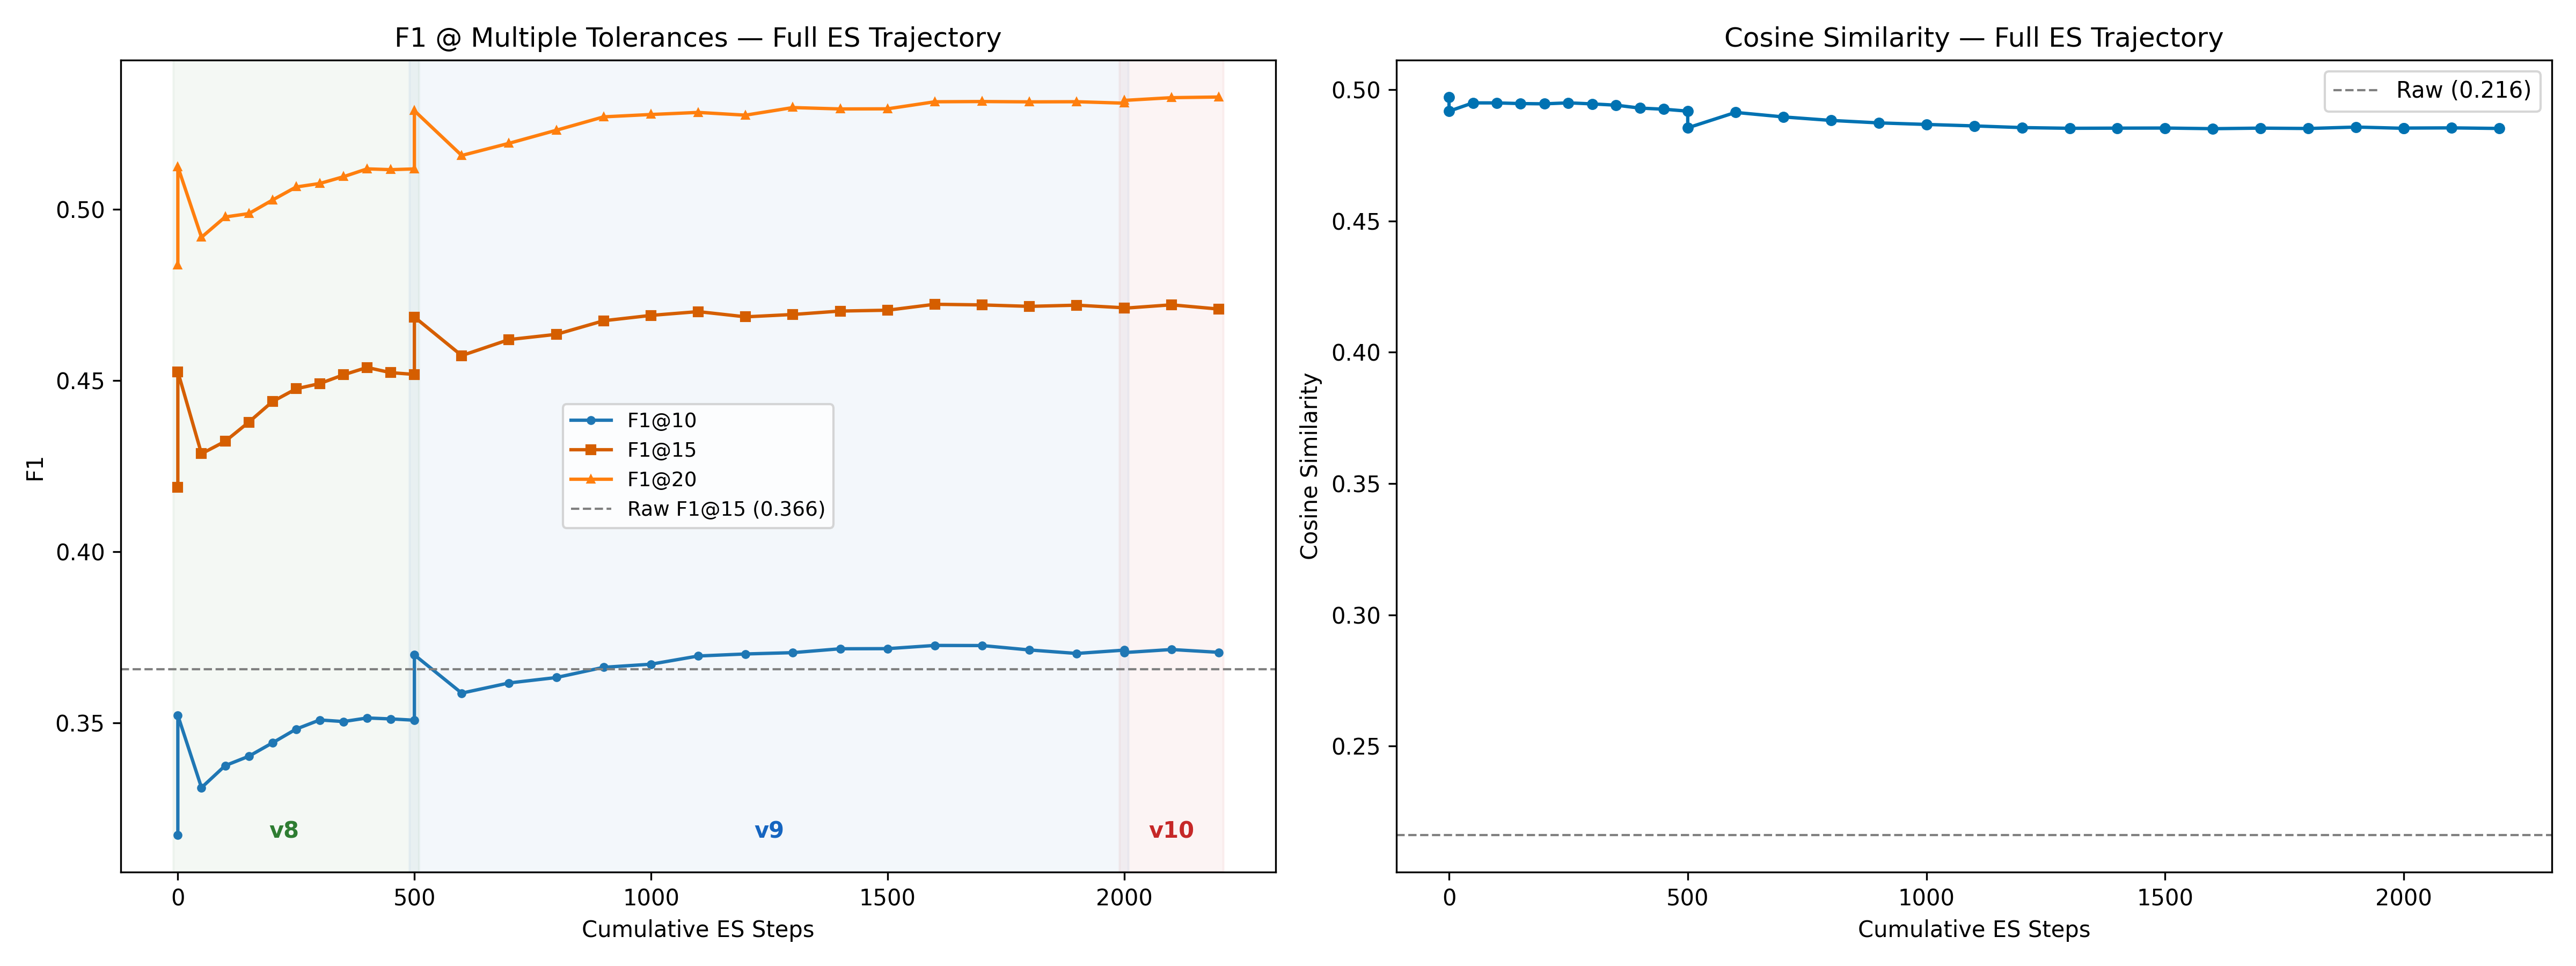
\includegraphics[width=\textwidth]{figures/fig_es_convergence.png}
    \caption{Evolution strategies convergence across ${\sim}$2000 cumulative steps. F1 at multiple tolerances improves monotonically in the fingerprint region. Version boundaries (v8$\to$v9$\to$v10) correspond to warm-start continuations with increased compute budget.}
    \label{fig:es-convergence}
\end{figure}

\begin{figure}[t]
    \centering
    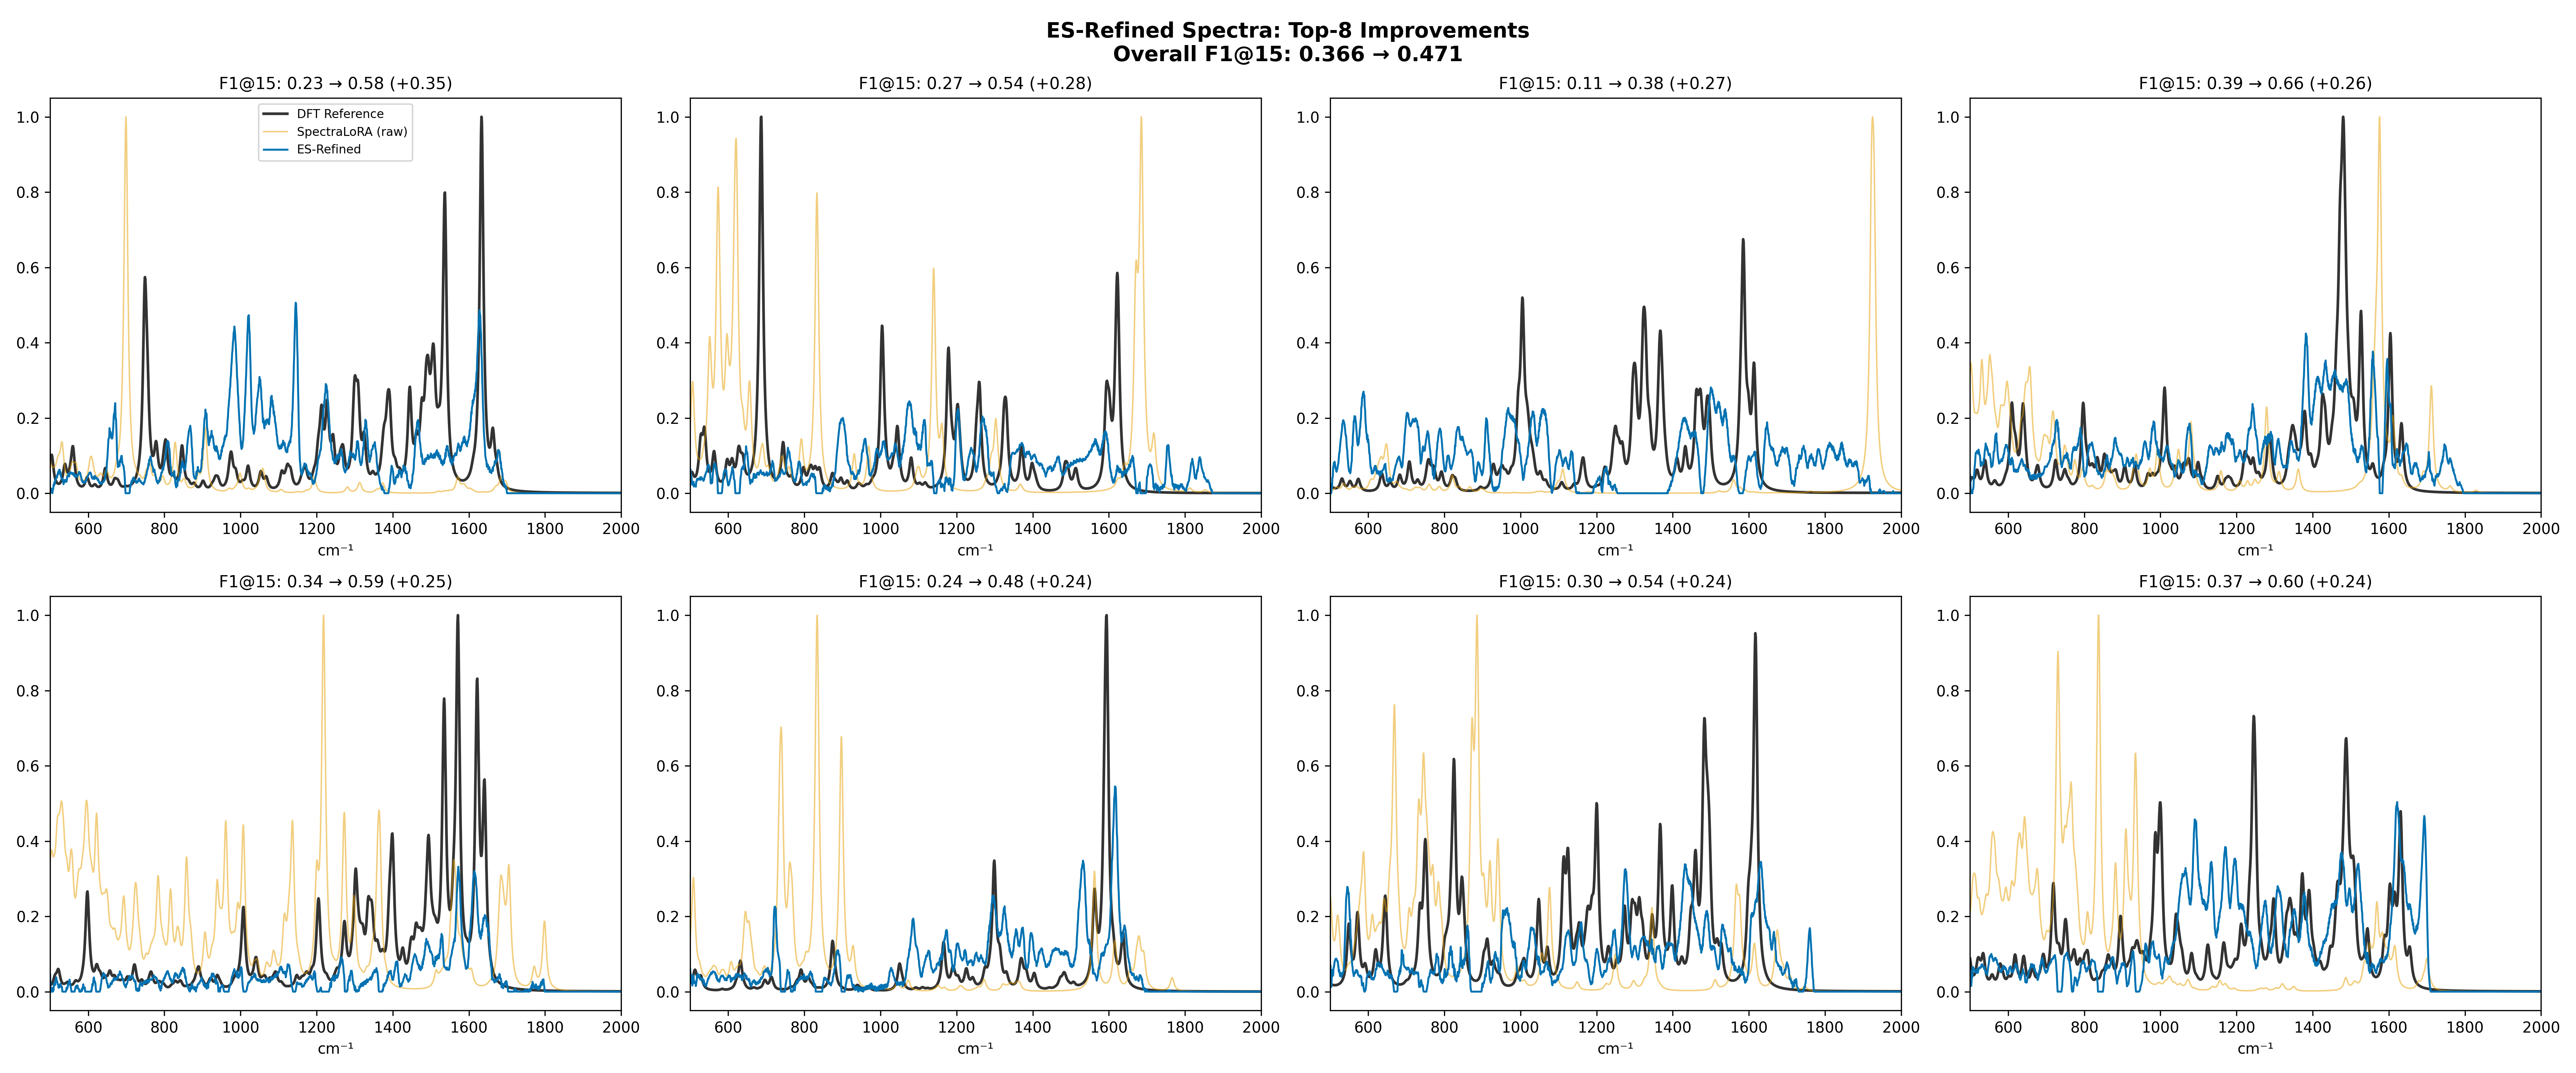
\includegraphics[width=\textwidth]{figures/fig_es_before_after.png}
    \caption{Before/after spectral refinement for the top-8 most improved test molecules. Black: DFT reference; orange: raw SpectraLoRA prediction; blue: ES-refined output. The refinement suppresses spurious peaks, sharpens real peaks, and improves spectral alignment without changing peak positions by more than ${\sim}$5~cm$^{-1}$.}
    \label{fig:es-before-after}
\end{figure}

\paragraph{Future directions.} The precision gap (0.440 vs.\ Mol2Raman's 0.629) identifies mode selection as the primary remaining bottleneck: the model predicts too many spectroscopically weak peaks that survive broadening. A dedicated mode-filtering head trained with DFT Raman activity supervision would directly address this. Better polarizability prediction, via explicit electron-density modeling or higher-order derivative targets, would address the underlying intensity bottleneck. Multi-fidelity training incorporating both DFT references and experimental spectra, and extension to peptides and proteins, are natural follow-ons.

%% ====================================================================
\section{Conclusion}
\label{sec:conclusion}
%% ====================================================================

SpectraLoRA demonstrates that a 9M-parameter equivariant molecular foundation model, adapted via parameter-efficient fine-tuning, can serve as a high-throughput surrogate for DFT dynamical matrices. On a blind, out-of-distribution benchmark of 1000 drug-like molecules, spanning elements and structural motifs absent from training, the model recovers 60.6\% of vibrational modes within $\pm 10$~cm$^{-1}$ with median positional error of 3.56~cm$^{-1}$, sufficient for thermochemical applications at linear cost. A post-hoc spectral refinement stage, combining peak-weighted RMSE pre-training with evolution strategies for direct F1 optimization, pushes fingerprint F1@15 from 0.426 to 0.532 and achieves 70.3\% peak recall, exceeding the in-distribution recall of the end-to-end Mol2Raman baseline on a substantially harder chemical domain. The precision gap (0.440 vs.\ 0.629) identifies mode selection as the specific target for future work.

\bibliography{main}
\bibliographystyle{tmlr}

\appendix
\section{DFT vibrational theory}
\label{sec:appendix-dft}

The molecular Hamiltonian within the Born--Oppenheimer approximation separates into nuclear and electronic parts: $\hat{H}_{\mathrm{mol}} = \hat{T}_n + \hat{H}_e(\mathbf{R})$, where the electronic Hamiltonian $\hat{H}_e$ depends parametrically on nuclear positions $\mathbf{R}$. The potential energy surface $E(\mathbf{R})$ is the ground-state eigenvalue of $\hat{H}_e$. Vibrational frequencies are obtained from the Hessian $H_{ia,jb} = \partial^2 E / \partial r_{ia}\,\partial r_{jb}$ evaluated at the equilibrium geometry. The Kohn--Sham DFT framework provides a tractable route to $E(\mathbf{R})$ by mapping the interacting many-electron problem to a fictitious non-interacting system with the same ground-state density, mediated by the exchange-correlation functional.

\section{Metric definitions}
\label{sec:appendix-metrics}

\begin{itemize}
    \item \textbf{Coverage@$\delta$}: a reference mode is covered if $\min_j |f_j^{\mathrm{pred}} - f_i^{\mathrm{ref}}| \leq \delta$.
    \item \textbf{Weighted coverage}: same, weighted by normalized reference intensity.
    \item \textbf{Matched-mode error}: $|\Delta\nu|$ computed only over successfully matched pairs within the tolerance.
    \item \textbf{Intensity MAE}: $|\log_{10}(I_{\mathrm{pred}}/I_{\mathrm{ref}})|$ over matched pairs, after per-molecule max normalization.
\end{itemize}

\end{document}
